\title{PS5 Solutions}

%TEMPLATE HEADER
%This is the homework solution template
\documentclass[11pt]{article}

%AMS-TeX packages
\usepackage{amssymb, amsmath, amsthm} 
\usepackage[margin=.75in]{geometry}
\usepackage{graphicx}
\usepackage{caption}
\usepackage{subcaption}
\usepackage{bm} % bold math
\usepackage{listings}
\usepackage{color} %red, green, blue, yellow, cyan, magenta, black, white
\definecolor{mygreen}{RGB}{28,172,0} % color values Red, Green, Blue
\definecolor{mylilas}{RGB}{170,55,241}

%Redefining sections as problems
\makeatletter
\newenvironment{problem}{\@startsection
       {section}
       {1}
       {-.2em}
       {-3.5ex plus -1ex minus -.2ex}
       {0.2ex plus .2ex}
       {\pagebreak[3]%forces pagebreak when space is small; use \eject for better results
       \Large\sc\noindent{Problem }}\\}
\makeatother

%Fancy-header package to modify header/page numbering 
\usepackage{fancyhdr}
\pagestyle{fancy}
\lhead{\textbf{Ge/ESE 118}} %name of the course
\chead{\textbf{}} %topic of the homework set
\rhead{\textbf{Solution 5}} %number of the homework set
\lfoot{}
\cfoot{}
\rfoot{\thepage}

%Include frequently used commands used for equations
%Fractions
\newcommand\fr[2]{\frac{#1}{#2}} %Regular fraction

%Braces, Brackets, Parentheses, etc.
\newcommand\brcs[1]{\{#1\}} %Braces
\newcommand\brckts[1]{\left[#1\right]} %Brackets
\newcommand\lr[1]{\left(#1\right)} %Parentheses
\newcommand\abs[1]{\Big\lvert#1\Big\rvert} %Absolute value
\newcommand\ltwo[1]{\lVert#1\rVert_2} %L2-norm
\newcommand\linf[1]{\lVert#1\rVert_\infty} %L2-norm

%Linear algebra
\newcommand\tr[1]{\text{tr}\left( \mathbf{#1}\right)} %Trace
\renewcommand\det[1]{\text{det}\left( \mathbf{#1}\right)} %Determinant

%Trigonometric & special functions
\newcommand\sinb[1]{\, \sin\left(#1\right)} %Sine with parentheses: sin(x)
\newcommand\cosb[1]{\, \cos\left(#1\right)} %Cosine with parentheses: cos(x)
\newcommand\tanb[1]{\, \tan\left(#1\right)} %Tangent with parentheses: tan(x)
\newcommand\cotb[1]{\, \cot\left(#1\right)} %Cotangent with parentheses: cot(x)
\newcommand\sinc[1]{\, \text{sinc}\left(#1\right)} %Sinc function: sinc = sin(x)/x

%Calculus
\renewcommand\d[1]{\, \text{d}#1} %Differential for integrals
\newcommand\der[2]{\frac{\text{d}#1}{\text{d}#2}} %Ordinary derivate first order
\newcommand\dder[2]{\frac{\text{d}^2#1}{\text{d}#2^2}} %Ordinary derivate second order
\newcommand\od[3]{\frac{\text{d}^{#3}#1}{\text{d}#2^{#3}}} %Ordinary derivate any order
\newcommand\pder[2]{\frac{\partial#1}{\partial#2}} %Partial derivate first order
\newcommand\pdder[2]{\frac{\partial^2#1}{\partial#2^2}} %Partial derivate second order
\newcommand\pd[3]{\frac{\partial^{#3}#1}{\partial#2^{#3}}} %Partial derivative any order

%Fourier transform
\newcommand\ft[1]{\hat{#1}} %Fourier coefficient

%Probability theory, Statistics
\newcommand\ex[1]{\mathbb{E}\left[#1\right]} %Expectation
\newcommand\pr[1]{\mathbb{P}\left(#1\right)} %Probability
\newcommand\Var[1]{\text{Var}\left(#1\right)} %Variance
\newcommand\Cov[1]{\text{Cov}\left(#1\right)} %Covariance
\newcommand\one{\mathbf{1}} %Unity

%Miscellaneous 
\renewcommand\mod{\text{mod}} %Modulo

%CONTENTS OF THE HW SET SOLUTION BEGIN HERE
\begin{document}
\lstset{language=Matlab,%
	  %basicstyle=\color{red},
  breaklines=true,%
  morekeywords={matlab2tikz},
  keywordstyle=\color{blue},%
  morekeywords=[2]{1}, keywordstyle=[2]{\color{black}},
  identifierstyle=\color{black},%}
  stringstyle=\color{mylilas},
  commentstyle=\color{mygreen},%
  showstringspaces=false,%without this there will be a symbol in the places where there is a space
  numbers=left,%
  numberstyle={\tiny \color{black}},% size of the numbers
  numbersep=9pt, % this defines how far the numbers are from the text
  emph=[1]{for,end,break},emphstyle=[1]\color{red}, %some words to emphasise
													  %emph=[2]{word1,word2}, emphstyle=[2]{style},    
}


\subsection*{Problem 1 (graded by Dunzhu \& Toby) X points}

\subsubsection*{(a) - 10 points}
Using the exact hessian, the result seems harder converge to global minimum,  starting from some initial guess. For example, in the following code, we perturb original ti to ti\_new, and starting from the original best guess, using approximate hessian and exact hessian we get
\begin{verbatim}
[Mapp, M] = 
          315.420926236077          981.798748762528
            29.13082945887         -3197.23151318091
         -15.9074484210616          2983.63633307186
          15.8359059771525         -638.182236017816
          5.25225424962686         -89.3648967235656
\end{verbatim}

The exact hessian converge to a local minimum, because the exact hessian is near singular at the initial guess, but the approximate hessian is much better. We can see the eigenvalue of those two hessian after the first iteration
\begin{verbatim}
[eigs(hess_app), eigs(hess)] =
          18.0176962395304          18.0254192403416
         0.098866195495413           0.1026429885873
        0.0037406745666659       0.00383013080700191
      3.13699101887875e-05      0.000138526270350115
      1.10844438320923e-05      6.51426797439541e-09
\end{verbatim}
Note the exact hessian has an eigenvalue about 6E-9, which causes larger shift from the initial guess
\begin{verbatim}
[hess_app\grad, hess\grad] =
       -0.281987601375779         -666.651385634329
          1.23392027564989          3227.54405527842
         -1.29604880279318         -3000.78453513507
         0.116870531211363          654.168962989986
        0.0190736135015402          94.6348252902216
\end{verbatim}


\lstinputlisting{hw1a.m}



\subsubsection*{(b) - 10 points}
\subsubsection*{(b.i)}
Change variable $t=1/\sigma$, then
\begin{eqnarray*}
\int_0^{\infty} \frac{1}{\sigma^N} \exp\left( -\frac{1}{2\sigma^2} A \right) d\sigma 
 & = &
 \int_0^{\infty} t^{N-2} \exp\left( -\frac{A}{2} t^2 \right) dt 
\end{eqnarray*}
Since
\begin{eqnarray*}
\int_0^{\infty} \exp\left( -\frac{A}{2} t^2 \right) dt = \sqrt{\frac{\pi}{2}} A^{-1/2} \propto A^{-1/2} \\
  \int_0^{\infty} t \exp\left( -\frac{A}{2} t^2 \right) dt = A^{-1} \propto A^{-1}
\end{eqnarray*}
Take derivative with respect to A, then
\begin{eqnarray*}
 \int_0^{\infty} \frac{-t^2}{2}\exp\left( -\frac{A}{2} t^2 \right) dt \propto A^{-1/2 -1} \\
  \int_0^{\infty} t \frac{-t^2}{2}\exp\left( -\frac{A}{2} t^2 \right) dt \propto A^{-1 -1} \\
\end{eqnarray*}
Continue this derivative, we have
\begin{eqnarray*}
 \int_0^{\infty} \left(\frac{-t^2}{2}\right)^{(N-2)/2}\exp\left( -\frac{A}{2} t^2 \right) dt \propto A^{-1/2 - (N-2)/2} 
\end{eqnarray*}
So
\begin{eqnarray*}
 \int_0^{\infty} t^{N-2}\exp\left( -\frac{A}{2} t^2 \right) dt \propto A^{-(N-1)/2} 
\end{eqnarray*}

\subsubsection*{(b.ii)}
Assume uniform prior, then
\begin{eqnarray*}
P(x,y | d ) &\propto & P( d | x,y)  =  \exp -F(x,y) \\
&= & \exp \left(
-F(x_0, y_0) 
- grad F|_{x_0,y_0} \cdot (x-x_0, y-y_0)'
 - \frac{1}{2} (x-x_0, y-y_0) H|_{x_0,y_0} (x-x_0, y-y_0)'
 \right)
\end{eqnarray*}

Since at $(x_0,y_0)$, $grad F = 0$, thus
\begin{eqnarray*}
P(x,y | d ) &\propto &
\exp \left(
 - \frac{1}{2} (x-x_0, y-y_0) H|_{x_0,y_0} (x-x_0, y-y_0)'
 \right)
\end{eqnarray*}

write $H$ as 
\begin{eqnarray*}
H= \begin{pmatrix}
A & B \\
B & C
\end{pmatrix}
\end{eqnarray*}
thus the joint pdf will be

\begin{eqnarray*}
f(x,y) = K \exp \left(
 - \frac{1}{2} [ A(x-x_0)^2 + 2B(x-x_0)(y-y_0) + C(y-y_0)^2 ]  
 \right)
\end{eqnarray*}
where $K$ is the constant that normalize the pdf, to get it, we have

\begin{eqnarray*}
\int_{-\infty}^{\infty} dy \int_{-\infty}^{\infty} dx f(x,y) & = &
\int_{-\infty}^{\infty} dy \int_{-\infty}^{\infty} dx 
K \exp \left(
 - \frac{1}{2} [ A(x-x_0)^2 + 2B(x-x_0)(y-y_0) + C(y-y_0)^2 ]  
 \right) \\
 & = &
 \int_{-\infty}^{\infty} dy \int_{-\infty}^{\infty} dx 
K \exp \left(
 - \frac{1}{2} [ Ax^2 + 2Bxy + Cy^2 ]  
 \right) \\
  & = &
 \int_{-\infty}^{\infty} dy \int_{-\infty}^{\infty} dx 
K \exp \left(
 - \frac{1}{2} [ A(x + By/A)^2 + (C - B^2/A)y^2 ]  
 \right) \\ 
   & = &
 \int_{-\infty}^{\infty} dy K \exp \left(
 - \frac{1}{2} (C - B^2/A)y^2
 \right)
 \int_{-\infty}^{\infty} dx 
\exp \left(
 - \frac{1}{2} [ A(x + By/A)^2 ]  
 \right) \\ 
    & = &
 \int_{-\infty}^{\infty} dy K \exp \left(
 - \frac{1}{2} (C - B^2/A)y^2
 \right)
 \int_{-\infty}^{\infty} dx 
\exp \left(
 - \frac{1}{2} Ax^2  
 \right) \\ 
    & = &
 \int_{-\infty}^{\infty} dy K \exp \left(
 - \frac{1}{2} (C - B^2/A)y^2
 \right) \sqrt{2\pi/A} \\
   & = &
 K \sqrt{2\pi/(C-B^2/A)}\sqrt{2\pi/A} \\
 & = & 2 \pi K / \sqrt{ A C - B ^2} \\
 & = & 1
\end{eqnarray*}

Now we want to show $E[x]=x_0$. This is true because  
\begin{eqnarray*}
E[x - x_0] & = & \int_{-\infty}^{\infty} dy \int_{-\infty}^{\infty} dx \quad
(x-x_0) f(x,y) \\
& \propto & \int_{-\infty}^{\infty} dy \int_{-\infty}^{\infty} dx \quad
(x-x_0)  \exp \left(
 - \frac{1}{2} [ A(x-x_0)^2 + 2B(x-x_0)(y-y_0) + C(y-y_0)^2 ]  
 \right) \\
 & \propto & \int_{-\infty}^{\infty} dy \int_{-\infty}^{\infty} dx \quad
x  \exp \left(
 - \frac{1}{2} [ Ax^2 + 2Bx(y-y_0) + C(y-y_0)^2 ]  
 \right) \\ 
  & \propto & \int_{-\infty}^{\infty} dy \int_{-\infty}^{\infty} dx \quad
x  \exp \left(
 - \frac{1}{2} [ Ax^2 + 2Bxy + Cy^2 ]  
 \right) \\ 
   & \propto & \int_{-\infty}^{\infty} dy \int_{-\infty}^{\infty} dx \quad
x  \exp \left(
 - \frac{1}{2} [ A(x + By/A) + (C-B^2/A)y^2 ]  
 \right) \\ 
    & \propto & \int_{-\infty}^{\infty} dy (By/A)
\exp \left(
 - \frac{1}{2} [ (C-B^2/A)y^2 ]  
 \right) \\
   & \propto & \int_{-\infty}^{\infty} dy \quad y
\exp \left(
 - \frac{1}{2} [ (C-B^2/A)y^2 ]  
 \right) \\ 
 & = & 0
\end{eqnarray*}
So similarly $E[y]=y_0$. 

Thus
\begin{eqnarray*}
\sigma_x^2 & = & E[(x-E[x])^2] \\
       & = & E[(x-x_0)^2] \\
       & = & \int_{-\infty}^{\infty} dy \int_{-\infty}^{\infty} dx \quad 
       \frac{\partial f(x,y)}{\partial A} /(-1/2) \\
       & = & 
       -2 \frac{\partial  }{\partial A} \int_{-\infty}^{\infty} dy \int_{-\infty}^{\infty} dx \quad 
        f(x,y) \\
       & = & 
       -2 \frac{\partial  }{\partial A} 2 \pi K / \sqrt{ A C - B ^2} \\
         & = & 
\frac{2\pi K}{(A-B^2/C)\sqrt{AC-B^2}} \\
& =  & \frac{C}{A C - B ^2}
\end{eqnarray*}
Similarly
\begin{eqnarray*}
\sigma_y^2& =  & \frac{A}{A C - B ^2}
\end{eqnarray*}

\begin{eqnarray*}
\sigma_{xy} & = & E[(x-E[x])(y-E[y])] \\
       & = & E[(x-x_0)(y-y_0)] \\
       & = & \int_{-\infty}^{\infty} dy \int_{-\infty}^{\infty} dx \quad 
       \frac{\partial f(x,y)}{\partial B} /(-1) \\
       & = & 
       - \frac{\partial  }{\partial B} \int_{-\infty}^{\infty} dy \int_{-\infty}^{\infty} dx \quad 
        f(x,y) \\       
& =  & \frac{-B}{A C - B ^2}
\end{eqnarray*}

Note that 
\begin{eqnarray*}
\begin{pmatrix}
A & B \\
B & C
\end{pmatrix}^{-1} 
= \frac{1}{AC-B^2}\begin{pmatrix}
C & -B \\
-B & A
\end{pmatrix}
\end{eqnarray*}
Thus we get what we want.

\subsection*{Problem 2 (graded by Dunzhu \& Toby) 20 points}
\subsubsection*{(b) (10 points)}
Here are some topics people mentioned about the ABT book:
\begin{itemize}
\item Appendix A, background knowledge
\item Number of data points vs number of model parameter, overdetermined, underdeterminined, mixed determinied
\item MAP and Bayes' theorem
\item L1 norm is better when existence of outlier
\item difficulty in inverse: existance, uniqueness, and instability
\item Fredholm integration equation of the first kind generalize many inverse problem
\item Chapter 11 Section 3, general multivarate normal case with prior
\item damped Newton's method, choose the step length instead of using full newton step
\item ABT mentioned p-values, chi-square statistics
\item in lecture, we maximize $P(d|m)$ to get the maximum likelihood, in ABT they defined $L(m|d) = P(d|m)$ first, then maximize it. ABT one is more clear, because $P(d|m)$ apprears to be a function of $d$, where in fact we want it to be a function of $m$. 
\end{itemize}

\subsubsection*{(c) (10 points)}
Here are some topics people mentioned:
\begin{itemize}
\item When estimating $\sigma^2$, devided by $N-1$ instead of $N$
\item Confused about $J(m)$ and $G(m)$, it's really the same thing, Jacobian 
\item class did a better job of describing prior
\item Class and ABT does not cover the case when prior is a given range
\item numerical calculation of derivative when it's hard to do it analytically
\item any method for finding global minimum?
\end{itemize}


\subsection*{Problem 3 (graded by Toby) 35 points}

\subsubsection*{(a) (5 points)}

The data $d_k$ are the measurements $u_k = (1.97, 1.81, 1.59, 1.44)^T \mathrm{ft s^{-1}}$. The model parameters are $\mathbf{m} = (u^*, z_0)^T$. We could have picked $\mathbf{m} = (\theta, z_0)^T$, but the former choice simplifies the calculations (see hint in problem statement). The model predictions are
\begin{equation}
g_k = \frac{u^*}{\kappa} \log \left( \frac{z_k+z_0}{z_0} \right).
\end{equation}
This solves problem part (a).

\subsubsection*{(b) (5 points)}

The squared error misfit function is often denoted as $\chi^2$ and is given by
\begin{equation}
\chi^2(\mathbf{m}) = \frac{1}{2}\sum_{k}\left(d_k - g_k(\mathbf{m})\right)^2.
\end{equation}
This function was sometimes called $F(\mathbf{m})$ in the lecture notes.
As derived in the lecture notes, for the Newton-method we need to calculate the $\mathbf{G}(\mathbf{m})$ matrix defined by the column vectors
\begin{subequations}
\begin{align}
G_{ku^*} &= \frac{1}{\kappa}\log\left(\frac{z_k + z_0}{z_0}\right),\, \forall k = 1, \hdots, 4\\
G_{kz_0} &= -\frac{u^*}{\kappa} \left( \frac{z_k}{z_0(z_k + z_0)} \right),\, \forall k = 1, \hdots, 4
\end{align}
\end{subequations}
with the simplified Hessian $\nabla \nabla \chi^2 (\mathbf{m}) \approx \mathbf{G}(\mathbf{m})^T\mathbf{G}(\mathbf{m})$ so that
\begin{equation}
\mathbf{m}_{n+1} = \mathbf{m}_n - \nabla \nabla \chi^2(\mathbf{m})^{-1} \left(\mathbf{d} -\mathbf{g}(\mathbf{m}) \right).
\end{equation}
Iteration with an approproate initial condition yields the best-fit answer. The MATLAB code is shown at the end of the solution set. We could have used the exact Hessian to calculate the best-fit answer, but the approximate Hessian perfroms well for reasonable initial conditions. The best-fit solution is \textbf{$u^* = 0.2025~\mathrm{ft s^{-1}}$ and $z_0 = 0.2394  ~\mathrm{ft}$}.

\subsubsection*{(c) (5 points)}

In this part of the problem we calculate the mean veclocity $U$ by integrating the velocity profile in the vertical. We have
\begin{subequations}
\begin{align}
U &= \frac{1}{H} \int_0^H u \d{z} = \frac{1}{H} \int_0^H \frac{u^*}{\kappa} \log \left( \frac{z_k+z_0}{z_0} \right) \d{z}\\
&= \frac{z_0}{H} \frac{u^*}{\kappa}\int_1^{\frac{H+z_0}{z_0}} \log \left( z' \right) \d{z'}\\
&= \frac{z_0}{H} \frac{u^*}{\kappa} \left[\frac{H+z_0}{z_0} \left[\log\left(\frac{H+z_0}{z_0} \right)-1\right]+1\right]\\
&= \frac{u^*}{\kappa} \left[\frac{H+z_0}{H} \log\left(\frac{H+z_0}{z_0} \right)-1\right]
\end{align}
\end{subequations}
Plugging in our best-fit parameter, we obtain an estimate as \textbf{$U = 1.5251~\mathrm{ft s^{-1}}$}. 

\subsubsection*{(d) (5 points)}

Because the model errors are assumed to be Gaussian, we obtain a Gaussian likelihood for the data $\mathbf{d} = (d_1, \hdots, d_N)^T$
\begin{equation}
p(\mathbf{d}|\mathbf{m}, \sigma)
= \frac{1}{(2\pi\sigma^2)^{N/2}} \exp\left( -\frac{\sum_{k=1}^N(d_k - \frac{u^*}{\kappa} \log \left( \frac{z_k+z_0}{z_0} \right))^2}{2\sigma^2} \right),
\end{equation}
where $N = 4$ is the number of data points. 
According to the lecture notes, marginalization with respect to $\sigma$ in the case of uniform priors for $\sigma$ yields a marginalized likelihood function of the form
\begin{equation}
p(\mathbf{d}|\mathbf{m}) \propto \left(\frac{1}{2}\sum_{k=1}^N(d_k - \frac{u^*}{\kappa} \log \left( \frac{z_k+z_0}{z_0} \right))^2\right)^{-\frac{N-1}{2}} = \exp(-F(\mathbf{m})),
\end{equation}
which defines the function $F(\mathbf{m})$ as
\begin{equation}
F(\mathbf{m}) = \frac{N-1}{2}\log \left[\frac{1}{2}\sum_{k=1}^N\left(d_k - \frac{u^*}{\kappa} \log \left( \frac{z_k+z_0}{z_0} \right)\right)^2\right] \equiv \frac{N-1}{2}\log\left[\chi^2(\mathbf{m})\right], 
\end{equation}
where $\chi^2(\mathbf{m})$ stands for squared error misfit.
Assuming uniform priors for $\mathbf{m}$ as well and using Bayes' theorem, we arrive at the posterior probability density function
\begin{equation}
p(\mathbf{m}|\mathbf{d}) = \frac{e^{-F(\mathbf{m})}}{\int \d{\mathbf{m}} e^{-F(\mathbf{m})}} = \frac{\left(\sum_{k=1}^N(d_k - \frac{u^*}{\kappa} \log \left( \frac{z_k+z_0}{z_0} \right))^2\right)^{-\frac{N-1}{2}}}{\int \left(\sum_{k=1}^N(d_k - \frac{u^*}{\kappa} \log \left( \frac{z_k+z_0}{z_0} \right))^2\right)^{-\frac{N-1}{2}} \d{\mathbf{m}}}, 
\end{equation}
where we also took into account the normalization factor.
As we have shown in class and on the homework sets before, because of the chain rule, the maximum a posteriori solution is given by the minimum of $F(\mathbf{m})$ and thus is equivalent to the least squares solution.
\begin{equation}
\nabla_\mathbf{m} p(\mathbf{m}|\mathbf{d}) \propto \nabla_\mathbf{m} F(\mathbf{m}) \propto \nabla_\mathbf{m} \chi^2(\mathbf{m})= 0.
\end{equation}
This is always the case if $F(\mathbf{m})$ is a strictly monotonic function of $\chi^2(\mathbf{m})$.

\subsubsection*{(e) (5 points)}

For the sample variance estimate $S^2$ at the maximum a posteriori parameter values $\mathbf{m}_0$ from the lecture notes and homework sets, we have
\begin{equation}
S^2 \approx \frac{2\chi^2(\mathbf{m}_0)}{N-1} = \frac{\sum_{k=1}^N(d_k - \frac{u^*_0}{\kappa} \log \left( \frac{z_k+z_{0_0}}{z_{0_0}} \right))^2}{N-1} \approx 1.958\cdot 10^{-3}~\mathrm{ft^2 s^{-2}}, 
\end{equation}
which similarly to previous homework sets gives an estimate for the data variance
\begin{equation}
\sigma^2 = \frac{S}{N} \approx 4.8950\cdot 10^{-4}~\mathrm{ft^2 s^{-2}}.
\end{equation}
Both of them are counted as appropriate answers to this question.

\subsubsection*{(f) (5 points)}
For this part of the problem, we are first going to derive the covariance matrix, by approximating the posterior probability distribution as a Gaussian. We can do that by expanding the exponent to second order around the maximum a posteriori parameter values $\mathbf{m}_0$. We then have
that
\begin{equation}
p(\mathbf{m}|\mathbf{d}) = \frac{e^{-F(\mathbf{m})}}{\int \d{\mathbf{m}} e^{-F(\mathbf{m})}}
\approx \frac{e^{-F(\mathbf{m_0})-\frac{1}{2}(\mathbf{m} - \mathbf{m}_0)^T\mathbf{H}(\mathbf{m_0})(\mathbf{m} - \mathbf{m}_0)}}{\int \d{\mathbf{m}} e^{-F(\mathbf{m_0})-\frac{1}{2}\mathbf{H}(\mathbf{m_0})(\mathbf{m} - \mathbf{m}_0)^2}}
=\frac{e^{-\frac{1}{2}(\mathbf{m} - \mathbf{m}_0)^T\mathbf{H}(\mathbf{m_0})(\mathbf{m} - \mathbf{m}_0)}}{2\pi\sqrt{\text{det}(\mathbf{H}(\mathbf{m_0})^{-1})}}
\end{equation}
As we have seen in class, the covariance matrix is given by the inverse of the Hessian of $F(\mathbf{m})$. In this case, we have
\begin{equation}
\mathbf{H}(\mathbf{m_0}) = \frac{N-1}{2\chi^2(\mathbf{m}_0)}\nabla\nabla \chi^2(\mathbf{m}_0)
\end{equation}, 
where $\nabla \nabla$ stands for the Hessian with respect to a function. From problem part (b), we already know that the Hessian of $\chi^2$ can be approximated as $\nabla\nabla\chi^2 =\mathbf{G}^T\mathbf{G}$ at the maximum a posteriori parameter values. Thus we arrive at the covariance matrix
\begin{equation}
\Sigma = \mathbf{H}(\mathbf{m_0})^{-1} = \frac{2\chi^2(\mathbf{m}_0)}{N-1}\left(\mathbf{G}(\mathbf{m}_0)^T\mathbf{G}(\mathbf{m}_0)\right)^{-1} = S^2 \left(\mathbf{G}(\mathbf{m}_0)^T\mathbf{G}(\mathbf{m}_0)\right)^{-1}.
\end{equation}
The values are calculated in the MATLAB script and are given by
\begin{equation}
\Sigma = 
\begin{pmatrix}
0.01161 & 0.00278\\
0.00278 & 0.00067
\end{pmatrix}
\end{equation}
in the appropriate units. This can be used to calculate an uncertainty estimate for the mean velocity $U$. We can perform a Taylor expansion of $U$ around the maximum a posteriori parameter values $\mathbf{m}_0$
\begin{subequations}
\begin{align}
U(\v{m}) &= U_0 + \nabla U_\v{m_0}\cdot(\v{m}-\v{m}_0) + \frac{1}{2}(\v{m}-\v{m}_0)^T\nabla \nabla U_\v{m_0}(\v{m}-\v{m}_0) + \mathcal{O}((\mathbf{m} - \mathbf{m}_0)^3)\\
U(\v{m})^2 &= U_0^2 + 2U_0\nabla U_\v{m_0}\cdot(\v{m}-\v{m}_0) + U_0(\v{m}-\v{m}_0)^T\nabla \nabla U_\v{m_0}(\v{m}-\v{m}_0)\\
&+ (\v{m}-\v{m}_0)^T\nabla U_\v{m_0}\nabla U_\v{m_0}^T\cdot(\v{m}-\v{m}_0)+ \mathcal{O}((\mathbf{m} - \mathbf{m}_0)^3).
\end{align}
\end{subequations}
Thus using the Gaussian approximation for the posterior probability distribution function the first moment of $U$ is given by
\begin{equation}
\ex{U} = \int \d{\v{m}} U(\v{m}) p(\v{m}|\v{d}) = U_0 + U_1 + \mathcal{O}((\mathbf{m} - \mathbf{m}_0)^4)
\end{equation}, 
where $U_1$ is just a place holder function. The second moment of $U$ is
\begin{subequations}
\begin{align}
\ex{U^2} &= \int \d{\v{m}} U^2(\v{m}) p(\v{m}|\v{d}) = U_0^2 + 2U_0U_1\\ 
&+ (\partial_{m_1}U)^2\Sigma_{m_1m_1}+ (\partial_{m_2}U)^2\Sigma_{m_2m_2}+ 2(\partial_{m_1}U\partial_{m_2}U)\Sigma_{m_1m_2} + \mathcal{O}((\mathbf{m} - \mathbf{m}_0)^4).
\end{align}
\end{subequations} 
Here we just carried out Gaussian integrations that have been treated on previous homework sets or in class. The approximations are valid, if the posterior probability distribution function is well approximated by a Gaussian (i.e, when $N$ is large) and when higher order terms in the Taylor expansions for $U$ and $U^2$ can be neglected. The variance of $U$ can then be approximated as
\begin{subequations}
\begin{align}
\sigma_U^2 = \Var{U} &= \ex{U^2} - \ex{U}^2 = (\partial_{m_1}U)^2\Sigma_{m_1m_1} + (\partial_{m_2}U)^2\Sigma_{m_2m_2}+ 2(\partial_{m_1}U\partial_{m_2}U)\Sigma_{m_1m_2}\\
&+ \text{higher order terms in 1/N}.
\end{align}
\end{subequations}
This is called the error propagation formalism (cf. Wikipedia). The value for $\sigma_U$ using the maximum a posteriori parameter values is
\begin{equation}
\sigma_U \approx 0.8082.
\end{equation}
Uncertainties can also be estimated using Monte Carlo simulations (as done on homework set 2), but the details of those simulations need to be specified and justified. The same is true for the grid search approach. Both of those alternative methods should yield uncertainties that are at most lower than the number above, as both of those methods solve the problem exactly.

\subsubsection*{(g) (5 points)}

From a physcal point of view, both $z_0$ and $u^*$ need to be positive in this setup. The river flows to the right and $z_0$ is the roughness legnth, which is a positive quantitiy that also ensures that the argument of the logarithm does not go to zero. The roughness length is a scaling parameter and usually small. For scaling parameters, we can use the prior $p(z_0) = 1/z_0$. Because it is unlikely that our model holds for waterfalls, we need to empahsize small angles $\theta$. For small angles $\sin(\theta) \approx \theta$ and thus $u^* \approx \sqrt{gH\theta}$. We could therefore pick a prior that emphasizes small $u^*$, for example $p(u^*) = 1/u^*$. For the posterior probability we find
\begin{equation}
p(\mathbf{m}|\mathbf{d}) = \frac{\left(\sum_{k=1}^N(d_k - \frac{u^*}{\kappa} \log \left( \frac{z_k+z_0}{z_0} \right))^2\right)^{-\frac{N-1}{2}}\frac{1}{z_0}\frac{1}{u^*}}{\int \left(\sum_{k=1}^N(d_k - \frac{u^*}{\kappa} \log \left( \frac{z_k+z_0}{z_0} \right))^2\right)^{-\frac{N-1}{2}} \frac{1}{z_0}\frac{1}{u^*} \d{u^*}\d{z_0}}.
\end{equation}
Then, a modified $F(\mathbf{m})$ is given by
\begin{equation}
F(\mathbf{m}) = \frac{N-1}{2}\log\left( \sum_{k=1}^N(d_k - \frac{u^*}{\kappa} \log \left( \frac{z_k+z_0}{z_0} \right))^2\right) + \log(z_0) + \log(u^*).
\end{equation}
Notice that optimizing this $F(\mathbf{m})$ is no longer equivalent to the least squares problem, because of the additional logarithmic terms. These two terms force the MAP solution to  emphasize small positive values of $u^*$ and $z_0$ and can be thought of as regularization terms.

\vspace{1cm}
\noindent Here is a plot of the profile:
\begin{figure}
\begin{center}
  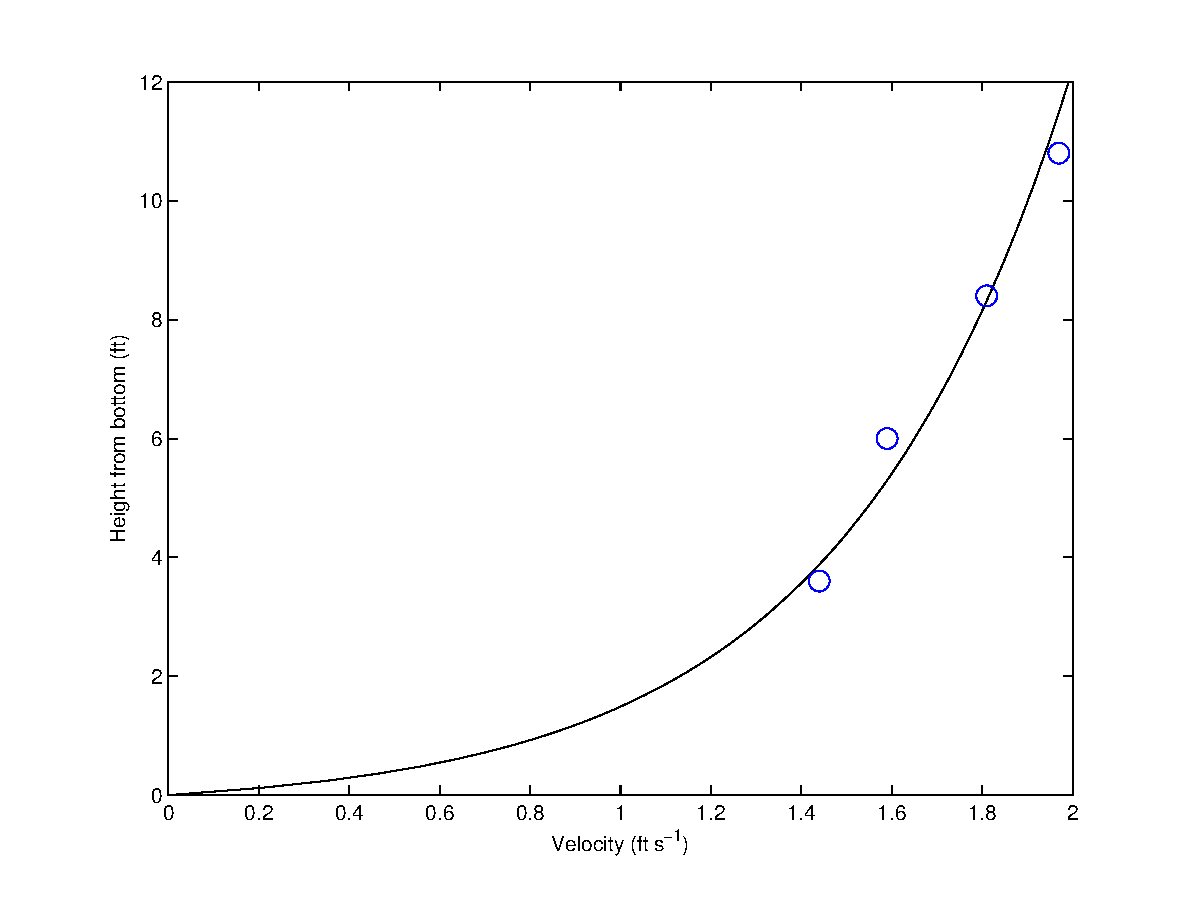
\includegraphics[width=12cm]{p3b.eps}
  \caption{(b): Prediction in black and data in blue for the flow profile. }
  \end{center}
\end{figure}


\vspace{1cm}
\noindent MATLAB code for this problem:
\begin{verbatim}
clc; clear all; close all;
%This script finds the best-fit model parameters and returns them and the
%covariance matrix. It also plots the date vs. the model prediction

%Problem part (b)
%Measurements / data
height = 12; %depth of the river
z = [0.9 0.7 0.5 0.3]'*height; %depths
v = [1.97 1.81 1.59 1.44]'; %velocity measurements

%Initialize the least squares method
z0 = 0.2; %Roughness length
u0 = 0.1; %Velocity amplitude
tol = 1e-15; %error tolerance for iteration close to machine accuracy

%Physical parameters that define the problem
kappa = 0.4; %von Karman constant

%Set up the parameter vector and initialize it
m = [z0 u0]';

%This is the iteration loop for the Newton algorithm
err = 0.2; %Initialize error. Break loop when error is small enough
while err > tol
    %Store old values
    m_old = m;
    
    %Calculate the G-matrix
    u = m(2)/kappa*log((z+m(1))/m(1));
    G = [-m(2)/kappa*z./(m(1)+z)/m(1), 1/kappa*log((z+m(1))/m(1))];
        
    %Calculate gradient and approximate Hessian for the Newton step
    H = G'*G;
    grad = -G'*(v-u);
    
    %Update model parameters using the Newton step
    m = m_old - inv(H)*grad;
    err = norm(m-m_old);
end

%Problem part (c)
%Calculate the  average velocity
U = m(2)/kappa*((height+m(1))/height*log((height+m(1))/m(1))-1);

%Problem part (e)
%Calculate variance and covariance matrix
N = length(z); %Number of data points
S = 1/(N-1)*sum((v-u).^2); %Sample variance
sigma2 = S/N; %Data variance estimate

%Problem part (f)
cov = S*inv(H); %Covariance matrix
sigmaU = sqrt((1/kappa*((height+m(1))/height*log((height+m(1))/m(1))-1))^2*cov(1,1) ...
          + (m(2)/kappa*(log((height+m(1))/m(1))-1/m(1)))^2*cov(2,2) ...
          + 2/kappa*((height+m(1))/height*log((height+m(1))/m(1))-1) ...
          * m(2)/kappa*(log((height+m(1))/m(1))-1/m(1))*cov(1,2));          

%Plot the predictions and the data
z_pred = (0:0.01:1)*height;
v_pred = m(2)/kappa*log((z_pred+m(1))/m(1));
plot(v_pred, z_pred, 'k-', v, z, 'bo', 'MarkerSize', 10);
xlabel('Velocity (ft s^{-1})');
ylabel('Height from bottom (ft)');
\end{verbatim}

\end{document}

